\documentclass[a4paper,10pt]{article}
%\usepackage[utf8x]{inputenc}
\usepackage[utf8]{inputenc}
\usepackage{graphicx}

%opening
\title{Automatic detection of bad habits of programming in Scratch}
\author{Jesús Moreno, Gregorio Robles}

\begin{document}

\maketitle

\begin{abstract}
This paper describes a method for automatic detection of two very bad programming habits present in students learning to program with Scratch, such as the repetition of code and object naming, and raises ideas to try to avoid such situations.

\end{abstract}

\section{Introduction}
Scratch \cite{resnick2009scratch}  is a programming environment that includes a visual programming language designed for children from 6 years old, a development environment and a website where the community can host their projects; run, study and reuse other programs; and share ideas or suggestions with other programmers. Although there are several similar visual programming languages, Scratch is undoubtedly the most successful and the one that is being used more regularly worldwide, with more than three million registered users on its website and more than five million shared project in its repository \footnote{http://scratch.mit.edu/statistics/}.
\paragraph{}Scratch is being used both in extracurricular activities \cite{maloney2008programming, kafai2010entering} or summer camps \cite{adams2010scratching, franklin2013assessment}, as in schools \cite{wilson2012evaluation}, high schools \cite{meerbaum2013learning} and even universities worldwide \cite{wolz2009starting, malan2007scratch}. Its capacity to bring computer programming to children and youth with the aim that in the future they would be willing to continue their studies in this discipline, and also its success to teach both basic and advanced programming concepts has been documented.
\paragraph{}However, it is also possible to find studies that have detected some bad programming habits in students learning to program in this environment \cite{meerbaum2011habits}. In this line, in our work as teachers we have detected other bad habits that, despite insisting our students to try to avoid them, we see how they are constantly repeated by pupils learning to program in Scratch. As these habits are contrary to the basic programming recommendations, our study tries to detect if they are also common in the projects shared on the Scratch repository and propose some ideas to try to avoid such situations.
\paragraph{}In section 2 a brief overview of Scratch is presented, works that study the learning demonstrated by students learning to program in this environment are reviewed, and studies that automate the evaluation of this learning are exposed. In section 3, our work methodology is described. Section 4 presents the obtained results. Finally, in section 5 the conclusions of our study are discussed and some ideas and suggestions for future work are provided.

\section{Background}

\paragraph{}Scratch is a visual programming environment developed by the Lifelong Kindergarten group at MIT Media Laboratory that allows to program interactive projects using a drag-and-drop approach with different pieces or \textit {Lego} style blocks \cite{resnick2009scratch}. Scratch was designed with the main goal of encouraging young people to program, and most of its users are novice learners with no prior programming experience \cite{maloney2010scratch}. The environment is designed to encourage users to manipulate and modify various media types, so that children and youth can create projects that they find interesting and attractive as animated stories, games or interactive presentations \cite{maloney2008programming}
\paragraph{}Scratch also offers a website where the projects programmed by the community are published, the code of each program can be studied, and it is possible to make suggestions and reuse the code of any project, so there are lots of valuable resources available for anyone willing to start to program. This approach also offers the opportunity to learn certain social skills related to programming, such as sharing and contributing to the community \cite{scaffidi2012skill}.
\paragraph{}As mentioned in the introduction, many papers showing that Scratch works as a tool for learning to program can be found \cite{maloney2008programming, franklin2013assessment, scaffidi2012skill, malan2007scratch}, as there are success stories in different educational levels, environments and disciplines showing that students learn concepts such as user interaction, conditional statements, communication and synchronization, logical expressions and data representation.
\paragraph{}Despite these good results, Meerbaum-Salant, Armoni and Ben-Ari \cite{meerbaum2011habits} prove that students learning to program in this environment show some bad habits that are contrary to recommended programming practices. In particular, they show excessive decomposition tendency and a development process absolutly from bottom to top starting with individual blocks of Scratch.
\paragraph{} Aiming to simplify the process of evaluating the Computational Thinking and help evaluators with an automation tool, Hairball was created \cite{boe2013hairball}. Hairball is a static analyzer of Scratch projects inspired by Lint \footnote{http:// www.unix.com/man-page/FreeBSD/1/lint} that tries to detect programming errors in Scratch projects, such as not initializing the value of a variable or the state of a character, sending messages that are not received by any program or including code that is never run.

\section{Methodology}

\paragraph{}In our work as teachers with high school students, we found that, despite our constant insistence and warnings to try to avoid them, many students show two bad habits in a regular basis that have to do with named object and code repetition.

\paragraph{}On the one hand, it is very common that students do not change the names of the characters, which are automatically named by the environment as \textit{SpriteX}, where X is an incremental number. When the aumount of characters in a project increases is quite hard to know which object relates to a given statement, contributing to poor code readability, slowing the project programming and complicating debugging for possible errors.
\paragraph{}On the other hand, it is also very common to see students repeat code in the same project, sometimes even in the same character programs. Thus, besides complicating the maintenance and updating of the code, the conceptss of abstraction and modularization, two key components of the development of computational thinking \cite{wing2008computational}, are not trained.
\paragraph{}In order to detect these two behaviors in Scratch projects, we have developed two plug-ins for the Hairball environment \cite{boe2013hairball}, which in turn makes use of kurt\textit{kurt}\footnote{https://github.com/blob8108/kurt}, a library implemented in python, to automate the detection of this type of bad practices in programs developed in this environment.
\paragraph{}The plug-in \textit{convention.SpriteNaming}\footnote{https://github.com/jemole/hairball/blob/master/hairball/plugins/convention.py} analyzes a Scratch project to check if the names of its characters begin with the string \textit{Sprite}, which indicates that the user has not changed its name and has left the one the system assigns by default to every new character added to the project.
\paragraph{}The plug-in \textit{duplicate.DuplicateScripts}\footnote{https://github.com/jemole/hairball/blob/master/hairball/plugins/duplicate.py} analyzes a Scratch project to try to locate repeated complete programs within a project. In order to do so the plug-in runs each project and gets the \textit{tokens} of the different blocks of the programs, so that two blocks that differ only in the received values are considered equal. To illustrate the operation of this plug-in, the picture \ref{fig:CodeRepetition1} shows two scripts containing the same blocks with the only difference of the velues received by parameter.
\begin{figure}
  \centering
    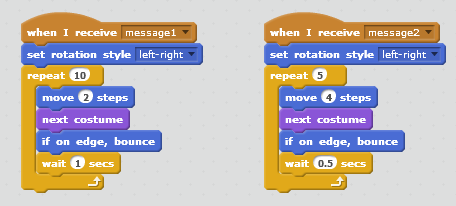
\includegraphics{img/CodeRepetition1.png}
  \caption{Two scripts repeating code}
  \label{fig:CodeRepetition1}
\end{figure}

\paragraph{}When these scripts are analyzed by the plug-in and translated into \textit{tokens} they would be considered equal, as their code would be translated to the next set of \textit{tokens}:
\begin{verbatim}
 'set rotation style %s'
 'repeat %s%s'
 'move %s steps'
 'next costume'
 'if on edge, bounce'
 'wait %s secs'
\end{verbatim}
\paragraph{}Thus, the correct way to implement this project would have been as shown in Figure \ref{fig:CodeRepetition2}, defining a new set of blocks that receives several values per parameter and reusing the block created in both programs. This solution would involve improvements regarding maintenance, updating and debugging.

\begin{figure}
  \centering
    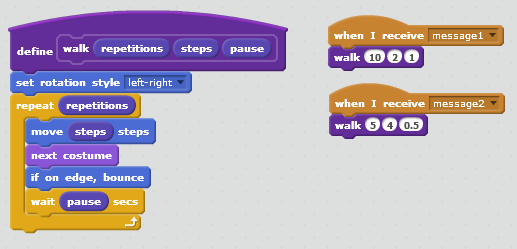
\includegraphics{img/CodeRepetition2.png}
  \caption{Defining own blocks to avoid code repetition}
  \label{fig:CodeRepetition2}
\end{figure}

\paragraph{}In order to test the functionality of the developed plug-ins and test whether these behaviors that we detected in our work are also repeated in the projects of the Scratch repository, we proceeded to download 100 projects from the repository. As the possibility for users to define their own blocks, using \textit{def\_block} block, is only available since the release of Scratch 2.0, downloaded projects were all created after that date.


\section{Findings}
\paragraph{}Data obtained after analyzing 100 downloaded projects confirm that observations made with our students are also very common in the community projects.
\paragraph{}Regarding the lack of habit of renaming the characters and not using the default name assigned by the environment, the 79 \% of the analyzed projects contained at least one \textit{SpriteX} character not renamed.
\paragraph{}As an example to illustrate the drawbacks associated with this malpractice, picture \ref{fig:SpriteNaming} shows a script that is difficult to read as it is necessary to explore the character area to find which character refers to a particular block, making it difficult to debug the code any problems should arise, making it hard to make any improvement in the code and even slowing down the programming time, as the name of the character must be memorized or checked every time a block is added. 
\begin{figure}
  \centering
    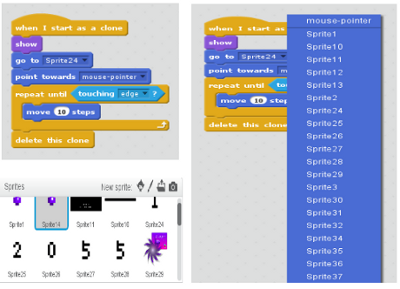
\includegraphics{img/SpriteNaming.png}
  \caption{Sprites with default names}
  \label{fig:SpriteNaming}
\end{figure}
\paragraph{}As for the repetition code, 62\% of the analyzed projects contained at least one repeated program. In fact, only 17\% of the analyzed projects made use of block \textit{def\_block} to define its own blocks that can be reused in other parts of the project. 

\section{Conclussions}

\paragraph{}Regarding the named object it is curious that Scratch users name correctly, ie significantly, the variables used in their projects. In our opinion the reason to explain this paradox is because it is mandatory to assign a name to a variable the moment it is created, as the environment does not name it by default. However, when creating a new character a  \textit{SpriteX} name is assigned automatically. A change on this feature of the environment, obliguing users to name new objects, would eliminate this malpractice.
\paragraph{}Regarding the code repetition and low usage Scratch users make of creating their own blocks (the equivalent of defining methods or procedures in other languages), works as the one performed by Seiter and Foreman \cite {seiter2013modeling}, in which they show that abstraction and modularization capacities are concepts that seem to be developed from a certain age, may explain the low rates of use of this functionality, since a significant part of the Scratch community consists of children under 10 years old \footnote{http://scratch.mit.edu/statistics/\#age}. Future studies should further investigate this line to continue advancing in the definition of an appropriate framework for different ages and to check whether users learning online and those who do it in a regulated environment show different use rates of this functionality .

\newpage
\bibliography{scratch}
\bibliographystyle{unsrt}
\end{document}
